\documentclass[presentation]{beamer}
\usepackage{../oop-slides-pianini}
\usepackage{ragged2e}
\usepackage{textcomp}
\usepackage{cleveref}
\setbeamertemplate{bibliography item}[text]
\author[Pianini]{Danilo Pianini\\Angelo Croatti, Simone Grotti, Mirko Viroli}
\title[L07 -- Eccezioni e Reflection]{L07 \\ Decentralized Version Control Systems, \\ Eccezioni e Interfacce grafiche}

\addtobeamertemplate{block begin}{}{\justifying}
\addtobeamertemplate{frame begin}{}{\justifying}

\begin{document}

\frame[label=coverpage]{\titlepage}

%====================
%Outline
%====================
% \fr{Outline}{
%   \bl{Goal della lezione}{
%     \iz{ 
% 			\item Sviluppo sinergico di codice in team
% 				\iz{
% 					\item Principi di base dei moderni sistemi di versioning
% 					\item Utilizzo locale di un Distributed Versions Control System
% 					\item Mercurial come esempio di DVCS
% 					\item Bitbucket come esempio di servizio per repository hosting
% 					\item Workflow suggeriti per lo sviluppo di progetti software
% 				}
% 			\item Definizione ed uso di nested class (quando necessario)
% 			\item Uso della Java Reflection API
% 			\item Definizione ed uso di enumerazioni (enum)
% 	  }
% 	}
% }

\begin{frame}<beamer>
 	\frametitle{Outline}
 	\tableofcontents[]
\end{frame}

\section{Decentralized version control systems I}

\subsection{Generalità}

\fr{Cosa sono}{
   I DVCS sono software che consentono di:
   \iz{
      \item Mantenere traccia dei cambiamenti fatti ad un progetto, consentendo di andare ``avanti e indietro'' nel tempo.
      \item Consentire e promuovere il lavoro di gruppo, anche in parallelo (lo vedremo nel prossimo lab)
   }

	L'esigenza di poter tornare a salvataggi precedenti è sempre stata avvertita dagli sviluppatori (e non solo). L'operazione di salvare più stati del proprio lavoro è detta \textit{versioning}, un software che semplifica il versioning è un \textit{version control system} (o \textit{versioning system}).
}

\fr{Pillole di storia}{

	Sistemi di versioning:
	\iz {
		\item ``Fai da te'' --- è il sistema che la maggior parte di voi ha usato finora: si fa una copia di tutti i file in una cartella (magari numerata). Costa molto in spazio ed in tempo, rende difficile lo scambio di file e il lavoro parallelo.
		\item \emph{CVS} --- Fu il primo sistema di versioning. Studiato per salvare automaticamente i punti di salvataggio di file di testo. È difficile usarlo per file binari, facilita lo scambio di file rispetto ad inviarsi cartelle.
		\item \emph{SVN} --- Evoluzione di CVS. Molto più veloce e con supporto nativo a file binari. Il lavoro in parallelo è possibile a patto di adottare un flusso di lavoro di squadra molto controllato.
		\item \emph{Git} e \emph{Mercurial} --- Sviluppati parallelamente per superare le limitazioni di SVN, sono nati praticamente identici. Più veloci di SVN e pensati per supportare il lavoro massivamente parallelo di team sparsi per il mondo.
	}
}

\fr{Diffusione}{
   Sono usati per (quasi) tutti i moderni processi di sviluppo software. Un po' di esempi:
   \iz{
      \item Android (git)
      \item Drupal (git)
      \item Facebook (Mercurial)
      \item GCC (git)
      \item Go (Mercurial)
      \item Java JDK (Mercurial)
      \item Libreoffice (git)
      \item Linux kernel (git)
      \item Nokia Maps (Mercurial)
      \item Python (Mercurial)
      \item VLC Video Player (git)
      \item Wine (git)
      \item le slides del prof. Viroli (Mercurial)
      \item le slides e le esercitazioni di laboratorio di OOP! (git)
   }
}

\fr{Diffusione}{
	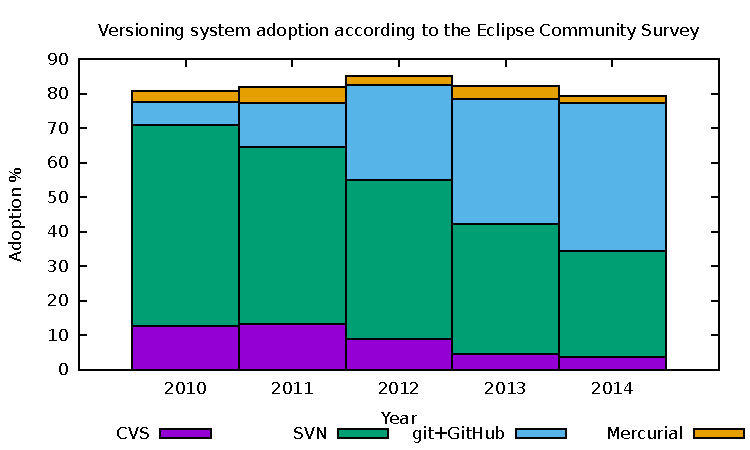
\includegraphics[width=\textwidth]{img/chart}
}

\begin{frame}{Mercurial vs. Git}
	\begin{block}{Similarità}
		\begin{itemize}
			\item Identici principi di base
			\item Spesso identici comandi
		\end{itemize}
	\end{block}
	\begin{block}{Principali differenze}
		\begin{itemize}
			\item Mercurial è concettualmente più snello, con architettura a plugin
			\item Git è più veloce, ha un'architettura monolitica
			\item Git gestisce il branching e gli accessi remoti in modo più semplice
			\item Git ha una gestione più conservativa dello ``stage''
			\item Git nasce per le esigenze di Linus Torvalds e Linux, e si porta dietro informazioni Unix-specifiche, come i permessi dei file
			\begin{itemize}
				\item Mercurial è più Windows-friendly...
				\item ...chi sviluppa in Unix tende a preferire le feature aggiuntive di Git
			\end{itemize}
		\end{itemize}
	\end{block}
	Imparato uno dei due sistemi, l'altro si apprende con un investimento di poche ore.
\end{frame}

\begin{frame}[fragile]{Bits of history}
	\begin{itemize}
		\item In April 2005, BitKeeper, the SCM Linux was developed with, withdrawn the free (as in beer) use
		\item No other SCM met the requirements of Torvalds
		\begin{itemize}
			\item Performance was the \textit{real} issue with such a code base
		\end{itemize}
		\item Torvalds decided to write his own
		\item The project was successful, and Torvalds appointed maintenance to Hamano
	\end{itemize}
	\begin{block}{Why the name}
		\begin{quote}
			I'm an egotistical bastard, and I name all my projects after myself. First 'Linux', now 'git'. \footnote{\tiny{From the project Wiki. ``git'' is slang for ``pig headed, think they are always correct, argumentative''}}
			\begin{flushright}
				\normalfont{--- Linus Torvalds}
			\end{flushright}
		\end{quote}
	\end{block}
\end{frame}

\begin{frame}[fragile]{The \texttt{git} \texttt{README.md} file}
	\begin{block}{}
		\begin{Verbatim}[fontsize=\footnotesize]
GIT - the stupid content tracker

"git" can mean anything, depending on your mood.

 - random three-letter combination that is pronounceable, and not
   actually used by any common UNIX command.  The fact that it is a
   mispronounciation of "get" may or may not be relevant.
 - stupid. contemptible and despicable. simple. Take your pick from the
   dictionary of slang.
 - "global information tracker": you're in a good mood, and it actually
   works for you. Angels sing, and a light suddenly fills the room. 
 - "goddamn idiotic truckload of sh*t": when it breaks
		\end{Verbatim}
	\end{block}
\end{frame}


\subsection{Concetti fondamentali}

\begin{frame}[allowframebreaks]{Concetti basilari e terminologia}
	\begin{block}{Repository}
		Il repository è l'insieme dei file che vengono tracciati dal DVCS assieme ai metadati, ossia alle informazioni che servono a ricostruire qualunque stato precedente.
	\end{block}
	\begin{block}{Tracciamento delle differenze}
		Abilità di registrare le differenze fra diverse versioni di uno o più file. Invece di salvare l'intero stato (tutto il contenuto di un file), vengono salvate solo le informazioni necessarie a ricostruire il file a partire dal salvataggio precedente
	\end{block}
	\begin{block}{Commit}
		Salvataggio dello stato del repository
	\end{block}
	\begin{block}{Staging area}
		Insieme delle modifiche accodate per esser salvate al prossimo commit. Il processo di salvataggio si articola infatti in due fasi:
		\begin{enumerate}
			\item \textbf{Staging} --- Selezione di quali file modificati, aggiunti o rimossi salvare al prossimo commit
			\item \textbf{Commit} --- Effettivo salvataggio delle modifiche presenti nella staging area
		\end{enumerate}
		Nota: Mercurial differisce da Git in questo particolare. Il concetto di staging area in Mercurial è assente, lo stato corrente del repository è esso stesso lo stage.
	\end{block}
	\begin{block}{Navigazione della storia}
		Possibilità di tornare ad un qualunque commit (salvataggio) precedente o successivo
	\end{block}
	\begin{block}{Branch}
		Linea di sviluppo (ossia sequenza di commit successivi). Dal momento in cui si può tornare indietro nella storia dei salvataggi e ripartire a sviluppare, si può creare una nuova linea di sviluppo, che si diparte da quella originale e procede parallelamente.
		\begin{center}
			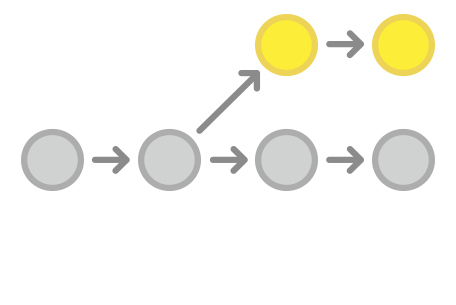
\includegraphics[height=.4\textheight]{img/branch}
		\end{center}
	\end{block}
	\begin{block}{Merge}
		Fusione di due branch (linee di sviluppo) in una sola.
		\begin{center}
			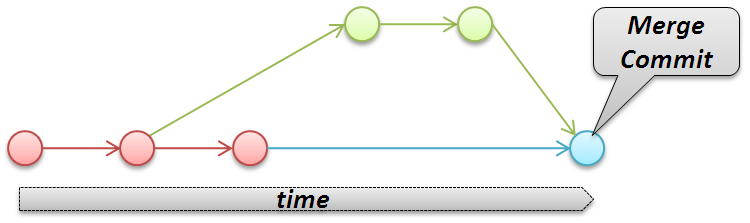
\includegraphics[width=.99\textwidth]{img/merge}
		\end{center}
	\end{block}
\end{frame}


\fr{Flussi di lavoro}{
  \bl{Branching} {
		Il branching è l'abilità di avviare nuove linee di lavoro a partire da un salvataggio precedente.
  }
  \bl{Merging} {
		Il merging è l'abilità di unire linee di lavoro separate in una unica.
  }
	\vspace{1cm}
	\centering 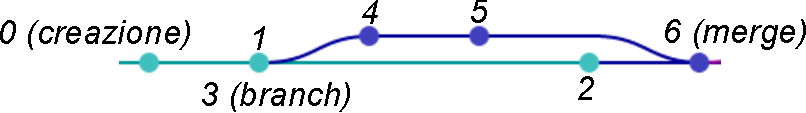
\includegraphics[width=0.99\textwidth]{img/flow0}
}

\subsection{Operazioni preliminari}

\begin{frame}[allowframebreaks]{Configurazione globale}
	\bl{In generale}{
		Come ogni prodotto software, i DVCS necessitano di alcune operazioni di configurazione preliminari. In particolare, richiedono di impostare un nome utente ed una email (in modo da poter capire chi ha apportato modifiche).
	}
	\bl{In Git}{
		È possibile specificare un nome utente di default utilizzando
		\iz {
			\item \texttt{git config --global user.name "YOUR NAME"}
			\begin{itemize}
				\item \textbf{OVVIAMENTE} al posto di \texttt{YOUR NAME} dovrete inserire il vostro nome.
			\end{itemize}
		}
		È possibile specificare una email di default utilizzando
		\iz {
			\item \texttt{git config --global user.email "your.email@provider"}
		}
	}
	\begin{block}{Esercizio}
		\begin{itemize}
			\item Si apra un terminale
			\item Si settino username ed email di default usando nome e cognome ed email istituzionale
		\end{itemize}
	\end{block}
\end{frame}

\section{Gestione di un repository}

\subsection{Operazioni di base sul repository}

\begin{frame}[allowframebreaks]{Inizializzazione di un repository}
	\bl{In generale}{
		È necessario esplicitare che, da un certo punto del file system, si desidera utilizzare il DVCS per tener traccia dei cambiamenti dei file contenuti da quel punto del file system.
	}
	\bl{In Git}{
		\iz{
			\item \texttt{git init}
		}
		Marca la cartella corrente come repository Git. Crea una sottocartella nascosta \texttt{.git} nella quale saranno salvati i metadati. Fintanto che la cartella \texttt{.git} è integra, sarà possibile ripristinare lo stato dei file del repository a qualunque versione.
		
		È possibile settare username ed email personalizzati per ogni repository, usando i comandi visti prima privati dell'argomento \texttt{--global}, e.g.:\\
		\begin{center}
			\texttt{git config user.email "your.second@email"}
		\end{center}
	}
	\begin{block}{Errori comuni}
		\begin{itemize}
			\item Bisogna posizionarsi dentro la cartella che ospiterà il nostro repository \textbf{prima} di dare il comando \texttt{git init}
			\item Dare il comando dentro la home folder (dove dovrebbe aprirsi il terminale di default) marcherà tutta la home folder come repository Git
		\end{itemize}
	\end{block}
	\begin{block}{Esercizio}
		\begin{itemize}
			\item Si crei una cartella di nome \texttt{dvcstest} (comando \texttt{mkdir})
			\item Si entri nella cartella col terminale
			\item Si inizializzi un repository git
			\item Si setti l'email utente \textbf{per il repository} al vostro indirizzo personale (quindi non quello \texttt{@studio.unibo.it})
			\begin{itemize}
				\item Nota: chi non volesse usare l'indirizzo personale per ragioni di privacy, usi una email fittizia.
			\end{itemize}
		\end{itemize}
	\end{block}
\end{frame}

\begin{frame}[allowframebreaks,fragile]{Ispezionare lo stato del repository}
	\begin{block}{In generale}
		È necessario sapere quale sia lo stato del repository e della staging area, per conoscere:
		\begin{itemize}
			\item Quali file sono stati modificati
			\item Quali file sono stati aggiunti allo stage
		\end{itemize}
	\end{block}
	\begin{block}{In Git}
		È possibile ispezionare lo stato usando:
		\begin{itemize}
			\item \texttt{git status}
		\end{itemize}
	\end{block}
	\begin{block}{Suggerimenti}
		\begin{itemize}
			\item Bisogna controllare spesso lo stato del repository
			\item Idealmente, prima di ogni operazione che potrebbe modificare lo stato del repository
		\end{itemize}
	\end{block}
	\begin{block}{Esercizio}
		\begin{itemize}
			\item Si ispezioni lo stato corrente del repository
		\end{itemize}
	\end{block}
	\begin{block}{Output atteso}
		\begin{Verbatim}[fontsize=\scriptsize]
On branch master

Initial commit

nothing to commit (create/copy files and use "git add" to track)		 
		\end{Verbatim}
	\end{block}
	\begin{block}{Spiegazione dell'output}
		\begin{itemize}
			\item Prima linea: il branch su cui ci si trova. Non ne è stato creato nessuno esplicitamente, quindi Git assume che di default si lavori su un branch di nome \texttt{master}
			\item Seconda linea: Git ci segnala che non abbiamo ancora effettuato alcun commit
			\item Terza linea: Git mostra lo stato della staging area. In questo momento non c'è nulla di cui far commit (difatti, non ci sono file nel nostro repository)
		\end{itemize}
	\end{block}
\end{frame}

\begin{frame}[allowframebreaks,fragile]{Aggiungere files alla staging area}
	\begin{block}{In generale}	
		È necessario segnalare esplicitamente quali file dovranno essere inclusi nel prossimo salvataggio.
		\begin{itemize}
			\item molti dei file potrebbero essere rigenerabili a partire da altri
			\item Il tracking differenziale è efficiente con file testuali...
			\item ...ma inefficiente con i binari!
			\item tracciare file generabili è uno spreco di risorse!
			\item I file selezionati saranno aggiunti alla ``staging area''
		\end{itemize}
	\end{block}
	\begin{block}{In un progetto Java}	
		Vanno tracciati:
		\begin{itemize}
			\item I sorgenti
			\item Le risorse (icone, file di configurazione...)
			\item Librerie jar copiate nel progetti (in realtà, vedrete in altri corsi, esistono sistemi migliori)
			\item Eventuali file esterni, ad esempio un README.md, un file per la licenza, il file .project di Eclipse per facilitare l'import...
		\end{itemize}
		\textbf{Non} vanno tracciati:
		\begin{itemize}
			\item I binari (rigenerabile dai sorgenti)
			\item La documentazione javadoc (rigenerabile dai sorgenti)
			\item I jar della vostra applicazione (rigenerabili)
		\end{itemize}
	\end{block}
	\begin{block}{In Git}
		Il sottocomando \texttt{add} aggiunge delle modifiche alla staging area
		\begin{itemize}
			\item \texttt{git add PATH\_TO\_FILE}
			\begin{itemize}
				\item Aggiunge il file indicato alla staging area. Il file deve essere all'interno del repository.
				\item Il file deve essere cambiato rispetto allo stato precedente (perché nuovo, modificato, o cancellato)
				\item Il file può essere un file che esisteva ma è stato cancellato!
				\item In questo caso, viene registrata nella staging area la cancellazione
			\end{itemize}
			\item \texttt{git add PATH\_TO\_FILE\_1 PATH\_TO\_FILE\_2 PATH\_TO\_FILE\_N}
			\begin{itemize}
				\item Aggiunge tutti i file indicati alla staging area.
			\end{itemize}
		\end{itemize}
	\end{block}
	\begin{block}{Esercizio}	
		\begin{itemize}
			\item All'interno della cartella dove abbiamo inizializzato il repository git vuoto, si creino due cartelle: \texttt{src} e \texttt{bin}
			\item Si crei dentro src un file \texttt{HelloWorld.java} (ad esempio con JEdit o Notepad++), contenente un semplice main con una stampa
			\item Si visualizzi lo stato del repository con \texttt{git status}
			\begin{itemize}
				\item Si noti che ci sono nuove informazioni!
				\item Git ci informa che ci sono dei file non tracciati dentro la cartella \texttt{src/}
			\end{itemize}
			\item Si utilizzi in modo appropriato il comando \texttt{git add} per aggiungere al tracking il file \texttt{HelloWorld.java}
			\item Se il comando viene eseguito correttamente, non viene dato alcun output all'utente
			\item Si visualizzi lo stato del repository
		\end{itemize}
	\end{block}
	\begin{block}{Output atteso}
		\begin{Verbatim}[fontsize=\scriptsize]
On branch master

Initial commit

Changes to be committed:
  (use "git rm --cached <file>..." to unstage)

        new file:   src/HelloWorld.java	 
			\end{Verbatim}
	\end{block}
	\begin{block}{Spiegazione dell'output}
		\begin{itemize}
			\item La parte relativa alla staging area è cambiata: git ci segnala che le modifiche ad \texttt{src/HelloWorld.java} saranno salvate al prossimo commit
		\end{itemize}
	\end{block}
\end{frame}

\begin{frame}[allowframebreaks,fragile]{Creare punti di salvataggio}
	\begin{block}{In generale}
		L'operazione fondamentale che vogliamo eseguire è quella di creare un punto di salvataggio, che registri i nostri progressi e al quale potremo sempre tornare.
		
		Assieme al salvataggio, vogliamo registrare alcuni metadati:
		\begin{itemize}
			\item Nome dell'autore del commit
			\item Informazioni per identificare e contattare l'autore (email)
			\item Un \textbf{messaggio} che riassuma quali modifiche sono state fatte in quel commit
			\item Data e ora del commit (acquisite automaticamente)
			\item Un identificativo univoco (hash) (generato automaticamente)
		\end{itemize}
		
		Il commit non salverà lo stato del progetto, ma il set di modifiche necessarie per portare i file dallo stato precedente a quello del nuovo commit.
	\end{block}
	\begin{block}{Buone pratiche di commit}
		È molto importante specificare un messaggio di commit sensato.
		\begin{itemize}
			\item Deve essere un breve riassunto di quanto è stato fatto dal salvataggio precedente
			\item Chi vede la storia del progetto deve capire immediatamente quali siano le differenze che il commit introduce
			\item È buona norma scrivere in inglese usando il simple present
		\end{itemize}
		È molto importante fare commit piccoli e frequenti
		\begin{itemize}
			\item Idealmente, uno ad ogni modifica di cui sia possibile fornire una descrizione organica nel commit message
			\item Non importa se le modifiche sono minimali
% 			\item Ad esempio, i seguenti sono buoni commit:
% 			\begin{itemize}
% 				\item \texttt{Aggiunta stampa in caso di errore}, con modifica di una sola linea di codice
% 				\item \texttt{Aggiunta di final mancanti}, con modifica di poche linee di codice in un solo file
% 				\item \texttt{Implementata versione iniziale della funzionalità X}, con modifica e aggiunta di diversi file sorgente
% 			\end{itemize}
		\end{itemize}
	\end{block}
	\begin{block}{Cattive pratiche da evitare}
		\begin{itemize}
			\item Messaggi non chiari, generici e/o troppo brevi, ad esempio:
			\begin{itemize}
				\item Fix bug
				\item Fix project
				\item Add files
				\item Commit
			\end{itemize}
			\item Commit giganteschi con molte modifiche, magari non strettamente correlate fra loro
		\end{itemize}
	\end{block}
	\begin{block}{In Git}
		Il sottocomando \texttt{commit} crea il salvataggio
		\begin{itemize}
			\item \texttt{git commit}
			\begin{itemize}
				\footnotesize
				\item Esegue un commit salvando tutte le modifiche nella staging area
				\item Apre l'editor di testo di sistema per l'inserimento del commit message
			\end{itemize}
			\item \texttt{git commit PATH\_TO\_FILE\_1 PATH\_TO\_FILE\_2 PATH\_TO\_FILE\_N}
			\begin{itemize}
				\footnotesize
				\item Esegue un commit salvando tutte le modifiche ai file elencati
				\item Apre l'editor di testo di sistema per l'inserimento del commit message
				\item Equivalente ad eseguire \texttt{git add FILES} seguito da \texttt{git commit} a partire da una staging area vuota
			\end{itemize}
			\item \texttt{git commit -m "A message"}
			\begin{itemize}
				\footnotesize
				\item Esegue un commit di tutte le modifiche aggiunte alla staging area
				\item Utilizza \texttt{A message} come commit message
			\end{itemize}
			\item \texttt{git commit FILES -m "A message"}
			\begin{itemize}
				\footnotesize
				\item Esegue un commit salvando tutte le modifiche ai file elencati
				\item Utilizza \texttt{A message} come commit message
			\end{itemize}
		\end{itemize}
	\end{block}
	\begin{block}{Configurare l'editor di testo}
		Sistemi diversi hanno editor diversi
		\begin{itemize}
			\item Di default MacOS X utilizza \texttt{vim}
			\item In Linux dipende dalla distribuzione, solitamente è uno fra \texttt{vim}, \texttt{nano}, o \texttt{emacs}
			\item In Windows \textit{dovrebbe} essere \texttt{Notepad.exe}
		\end{itemize}
		Non sempre l'editor di default è quello che preferite: è bene configurarlo
		\begin{itemize}
			\item \texttt{git config --global core.editor "editorcommand"}
			\begin{itemize}
				\item Setta \texttt{editorcommand} come comando da invocare per aprire l'editor
				\item Va da sé che il comando debba essere disponibile sul vostro sistema...
			\end{itemize}
		\end{itemize}
		Vi consiglio di:
		\begin{itemize}
			\item Se conoscete già un editor a command line, usate quello
			\item Se non lo avete, in ambiente Linux o Mac, di usare \texttt{nano}
		\end{itemize}
	\end{block}
	\begin{block}{Esercizio}	
		\begin{itemize}
			\item Se si sta usando Linux o MacOS X, si configuri adeguatamente l'editor di testo
			\item Si verifichi lo stato del repository
			\item Si effettui il commit delle modifiche presenti nella staging area
			\begin{itemize}
				\item Inserendo un commit message SENSATO!
			\end{itemize}
			\item Si visualizzi lo stato del repository
		\end{itemize}
	\end{block}
	\begin{block}{Output atteso dopo il commit}
		\begin{Verbatim}[fontsize=\scriptsize]
[master (root-commit) 19aa252] Create HelloWorld
 1 file changed, 5 insertions(+)
 create mode 100644 src/HelloWorld.java
\end{Verbatim}
	\end{block}
	\begin{block}{Spiegazione dell'output}
		\begin{itemize}
			\item Ci troviamo nel branch master
			\item Questo è il primo commit (radice)
			\item L'hash del nostro commit (una parte, in realtà) è \texttt{19aa252}
			\begin{itemize}
				\item Ovviamente il vostro potrebbe differire
			\end{itemize}
			\item Il messaggio inserito è ``Create HelloWorld''
			\begin{itemize}
				\item Ovviamente questo è il mio, il vostro potrebbe essere diverso, dipende da che messaggio avete inserito
			\end{itemize}
			\item È stato modificato un file, in totale sono state inserite 5 righe di codice
			\item È stato creato un nuovo file \texttt{src/HelloWorld.java}
			\begin{itemize}
				\item Si noti che sono stati tracciati i permessi unix (\texttt{644} in ottale)
			\end{itemize}
		\end{itemize}
	\end{block}
\end{frame}

\begin{frame}[allowframebreaks,fragile]{Rimuovere files dalla staging area}
	\begin{block}{In generale}	
		Vogliamo poter togliere dalla staging area dei file che abbiamo aggiunto
		\begin{itemize}
			\item Ad esempio perché li abbiamo aggiunti a seguito dell'uso di un comando con la wildcard
			\item Oppure perché abbiamo deciso di salvare le modifiche in più commit
		\end{itemize}
	\end{block}
	\begin{block}{In Git}
		Il sottocomando \texttt{reset} rimuove delle modifiche dalla staging area
		\begin{itemize}
			\item \texttt{git reset PATH\_TO\_FILE}
			\begin{itemize}
				\item Rimuove le modifiche fatte al file selezionato dalla staging area (non dal tracking!)
				\item Il file potrebbe anche non esistere, ad esempio se abbiamo cancellato un file e aggiunto la modifica alla staging area.
			\end{itemize}
			\item \texttt{git reset PATH\_TO\_FILE\_1 PATH\_TO\_FILE\_2 PATH\_TO\_FILE\_N}
			\begin{itemize}
				\item Rimuove le modifiche fatte a tutti i file indicati dalla staging area.
			\end{itemize}
		\end{itemize}
	\end{block}
\end{frame}

\subsection{Gestione dei file}

\begin{frame}[allowframebreaks,fragile]{Ignorare file indesiderati}
	\begin{block}{In generale}
		In molti casi, vorremmo poter dire al DVCS di ignorare alcuni file o cartelle, che sappiamo essere rigenerabili o che riteniamo non utili
		\begin{itemize}
			\item I file compilati
			\item I file contenenti la Javadoc
			\item I nostri jar
		\end{itemize}
	\end{block}
	\begin{block}{In Git}
		È possibile creare, nella radice del repository, un file \texttt{.gitignore}
		\begin{itemize}
			\item I file elencati dentro \texttt{.gitignore} saranno invisibili a Git
			\item È bene che il file \texttt{.gitignore} venga aggiunto al tracker!
		\end{itemize}
	\end{block}
	\begin{block}{Sintassi di .gitignore}
		\begin{Verbatim}[fontsize=\scriptsize]
bin/
doc/
*.log
*.pdf
!myImportantFile.pdf
		\end{Verbatim}
		Stiamo dicendo che git deve:
		\begin{itemize}
			\item Ignorare la cartella \texttt{bin}, e tutto il suo contenuto
			\item Ignorare la cartella \texttt{doc}, e tutto il suo contenuto
			\item Ignorare tutti i file di con estensione \texttt{.log}
			\item Ignorare tutti i file di con estensione \texttt{.pdf}
			\item Non ignorare il file \texttt{myImportantFile.pdf}
			\begin{itemize}
				\item È possibile usare \texttt{!} per creare eccezioni ad una regola
				\item È molto più comodo che elencare tutti i file da escludere uno per uno!
			\end{itemize}
		\end{itemize}
	\end{block}
	\begin{block}{Note sulla creazione di file il cui nome inizia per \texttt{.}}
		\begin{itemize}
			\item Windows ha l'abitudine di aggiungere autonomamente l'estensione ai file che vengono creati...
			\item ...per poi nasconderla
			\item Verificate \textbf{sempre con il terminale} che il file sia esattamente quello che vi aspettate, ossia \texttt{.gitignore}
			\item Se il file viene chiamato \texttt{.gitignore.txt}, o in qualunque modo diverso da \texttt{.gitignore}, non sarà considerato un ignore file valido da Git!
		\end{itemize}
		Il problema non si pone su MacOS X e Linux.
	\end{block}
	\begin{block}{Esercizio}	
		\begin{itemize}
			\item Si compili dentro bin il file HelloWorld.java che avete creato
			\begin{itemize}
				\item Spero che vi ricordiate come si compila un file con \texttt{javac}
				\item Se il file non compilasse, sistematelo, quindi aggiungetelo alla staging area ed eseguite un commit
				\item Già che ci siamo, eseguite e verificate che funzioni
			\end{itemize}
			\item Si osservi lo stato del repository
			\item Si crei un file \texttt{.gitignore} che ignori la cartella bin e tutto il suo contenuto
			\item Si osservi lo stato del repository
			\item Si aggiunga \texttt{.gitignore} alla staging area
			\item Si osservi lo stato del repository
			\item Si effettui il commit
			\item Si osservi lo stato del repository
		\end{itemize}
	\end{block}
	\begin{block}{Output atteso: primo \texttt{git status}}
		\begin{Verbatim}[fontsize=\scriptsize]
On branch master
Untracked files:
  (use "git add <file>..." to include in what will be committed)

        bin/

nothing added to commit but untracked files present (use "git add" to track)
		\end{Verbatim}
	\end{block}
	\begin{block}{Output atteso: secondo \texttt{git status}}
		\begin{Verbatim}[fontsize=\scriptsize]
On branch master
Untracked files:
  (use "git add <file>..." to include in what will be committed)

        .gitignore

nothing added to commit but untracked files present (use "git add" to track)
		\end{Verbatim}
	\end{block}
	\begin{block}{Output atteso: terzo \texttt{git status}}
		\begin{Verbatim}[fontsize=\scriptsize]
On branch master
Changes to be committed:
  (use "git reset HEAD <file>..." to unstage)

        new file:   .gitignore

		\end{Verbatim}
	\end{block}
	\begin{block}{Output atteso: commit}
		\begin{Verbatim}[fontsize=\scriptsize]
[master 3ae8422] Create .gitignore
 1 file changed, 1 insertion(+)
 create mode 100644 .gitignore
		\end{Verbatim}
	\end{block}
	\begin{block}{Output atteso: quarto \texttt{git status}}
		\begin{Verbatim}[fontsize=\scriptsize]
On branch master
nothing to commit, working tree clean
		\end{Verbatim}
	\end{block}
	\begin{block}{Spiegazione dell'output}
		\begin{itemize}
			\item Si noti come \texttt{bin/} sparisca dai file presenti nell'area di lavoro una volta che il file \texttt{.gitignore} è stato creato
		\end{itemize}
	\end{block}
\end{frame}

\begin{frame}[allowframebreaks,fragile]{Rimozione e rinominazione}
	\begin{block}{In generale}
		Vogliamo poter cancellare e rinominare files, e tracciare il fatto che lo abbiamo fatto
	\end{block}
	\begin{block}{In Git}
		Git è in grado di capire da solo quando qualcosa è stato modificato o eliminato (in questo è molto più semplice di Mercurial)
		\begin{itemize}
			\item Git tratta tutte le modifiche allo stesso modo
			\item A fronte della cancellazione di un file, basta aggiungerlo alla staging area perché la modifica venga registrata al successivo commit
			\item A fronte di una rinominazione, si aggiungono sia il file col vecchio nome che quello col nuovo
			\begin{itemize}
				\item Diversamente, verrà trattata come una rimozione o un'aggiunta, a seconda di quale delle due modifiche aggiungete all'area di staging.
			\end{itemize}
		\end{itemize}
	\end{block}
	\begin{block}{Esercizio}	
		Premessa: si osservi lo stato del repository con \texttt{git status} \textbf{prima e dopo ogni operazione}, assicurandosi di capire appieno l'output fornito da Git
		\begin{itemize}
			\item Si crei un file \texttt{junk.txt}, con un contenuto casuale
			\item Si aggiunga \texttt{junk.txt} alla staging area
			\item Si effettui il commit
			\item Si rinomini \texttt{junk.txt} in \texttt{trash.txt}
			\item Si aggiungano tutte le modifiche alla staging area
% 			\begin{itemize}
% 				\item Protip: \texttt{git add *}
% 				\item Da usare il \textit{meno possibile}! È un comando \textit{potenzialmente dannoso}!
% 			\end{itemize}
			\item Si effettui il commit
			\item Si elimini \texttt{trash.txt}
			\item Si aggiunga \texttt{trash.txt} alla staging area
			\item Si effettui il commit
		\end{itemize}
	\end{block}
	\begin{block}{Output atteso 1}
		\begin{Verbatim}[fontsize=\scriptsize]
On branch master
Untracked files:
  (use "git add <file>..." to include in what will be committed)

        junk.txt

nothing added to commit but untracked files present (use "git add" to track)
		\end{Verbatim}
	\end{block}
	\begin{block}{Output atteso 2}
		\begin{Verbatim}[fontsize=\scriptsize]
On branch master
Changes to be committed:
  (use "git reset HEAD <file>..." to unstage)

        new file:   junk.txt

		\end{Verbatim}
	\end{block}
	\begin{block}{Output atteso 3}
		\begin{Verbatim}[fontsize=\scriptsize]
[master 844aebd] Add junk
 1 file changed, 1 insertion(+)
 create mode 100644 junk.txt
		\end{Verbatim}
	\end{block}
	\begin{block}{Output atteso 4}
		\begin{Verbatim}[fontsize=\scriptsize]
On branch master
Changes not staged for commit:
  (use "git add/rm <file>..." to update what will be committed)
  (use "git checkout -- <file>..." to discard changes in working directory)

        deleted:    junk.txt

Untracked files:
  (use "git add <file>..." to include in what will be committed)

        trash.txt

no changes added to commit (use "git add" and/or "git commit -a")
		\end{Verbatim}
	\end{block}
	\begin{block}{Output atteso 5}
		\begin{Verbatim}[fontsize=\scriptsize]
On branch master
Changes to be committed:
  (use "git reset HEAD <file>..." to unstage)

        renamed:    junk.txt -> trash.txt

		\end{Verbatim}
	\end{block}
	\begin{block}{Output atteso 6}
		\begin{Verbatim}[fontsize=\scriptsize]
[master 4d086a9] move junk to trash
 1 file changed, 0 insertions(+), 0 deletions(-)
 rename junk.txt => trash.txt (100%)
		\end{Verbatim}
	\end{block}
	\begin{block}{Output atteso 7}
		\begin{Verbatim}[fontsize=\scriptsize]
On branch master
Changes not staged for commit:
  (use "git add/rm <file>..." to update what will be committed)
  (use "git checkout -- <file>..." to discard changes in working directory)

        deleted:    trash.txt

no changes added to commit (use "git add" and/or "git commit -a")

		\end{Verbatim}
	\end{block}
	\begin{block}{Output atteso 8}
		\begin{Verbatim}[fontsize=\scriptsize]
[master 47b5f2f] Remove the trash
 1 file changed, 1 deletion(-)
 delete mode 100644 trash.txt

		\end{Verbatim}
	\end{block}
	\begin{block}{Output atteso 9}
		\begin{Verbatim}[fontsize=\scriptsize]
On branch master
nothing to commit, working tree clean
		\end{Verbatim}
	\end{block}
\end{frame}

\subsection{Visualizzazione della linea di sviluppo}

\begin{frame}[allowframebreaks,fragile]{Visualizzazione della storia}
	\begin{block}{In generale}
		Visualizzare l'elenco dei commit effettuati, chi li ha eseguiti, quando, ed il loro message commit
	\end{block}
	\begin{block}{In Git}
		Git offre il sottocomando \texttt{log}
		\begin{itemize}
			\item \texttt{git log}
			\begin{itemize}
				\item Visualizza tutti i commit della linea di sviluppo corrente
				\item Se l'output è troppo lungo crea una visualizzazione scorrevole (si vedano i comandi Unix \texttt{less} e \texttt{more})
				\item Per uscire dalla visualizzazione scorrevole, si usa il tasto Q
			\end{itemize}
			\item \texttt{git log --graph}
			\begin{itemize}
				\item Come sopra, con visualizzazione grafica dell'evoluzione sulla sinistra 
			\end{itemize}
		\end{itemize}
	\end{block}
	\begin{block}{Esercizio}	
		\begin{itemize}
			\item Si visualizzi l'attuale storia del repository, corredata di grafico
		\end{itemize}
	\end{block}
	\begin{block}{Output atteso}
		\begin{Verbatim}[fontsize=\tiny]
* commit 47b5f2fb9f5300dc8bc530ce45d37a86a0436755
| Author: Danilo Pianini <danilo.pianini@unibo.it>
| Date:   Wed Oct 19 16:46:21 2016 +0200
| 
|     Remove the trash
|  
* commit 4d086a9b0d2139f0cd300d329f532a2c464304c7
| Author: Danilo Pianini <danilo.pianini@unibo.it>
| Date:   Wed Oct 19 16:45:28 2016 +0200
| 
|     move junk to trash
|  
* commit 844aebd840e6f3d2b034312e9fa37677f64b9a15
| Author: Danilo Pianini <danilo.pianini@unibo.it>
| Date:   Wed Oct 19 16:43:48 2016 +0200
| 
|     Add junk
|  
* commit 3ae84225f45afdfa02c268c6079e0f6c96695c1f
| Author: Danilo Pianini <danilo.pianini@unibo.it>
| Date:   Wed Oct 19 16:26:30 2016 +0200
| 
|     Create .gitignore
|  
* commit 19aa252373d1e44897233bf5b733cf82019cd5bf
  Author: Danilo Pianini <danilo.pianini@unibo.it>
  Date:   Wed Oct 19 15:51:10 2016 +0200
  
      Create HelloWorld
		\end{Verbatim}
	\end{block}
\end{frame}

\begin{frame}[allowframebreaks,fragile]{Visualizzazione delle differenze}
	\begin{block}{In generale}
		Vogliamo poter controllare quali modifiche sono state introdotte da un commit
	\end{block}
	\begin{block}{In Git}
		Git può mostrare le modifiche fra intercorse fra due commit col sottocomando \texttt{diff}
		\begin{itemize}
			\item \texttt{git diff}
			\begin{itemize}
				\item Mostra le differenze fra l'ultimo commit effettuato e il contenuto della staging area
			\end{itemize}
			\item \texttt{git diff FROM}
			\begin{itemize}
				\item Dove \texttt{FROM} è lo hash di un commit
				\item Mostra le differenze fra \texttt{FROM} e la staging area
			\end{itemize}
			\item \texttt{git diff FROM TO}
			\begin{itemize}
				\item Dove \texttt{FROM} e \texttt{TO} sono gli hash di due commit
				\item Mostra le differenze fra \texttt{FROM} e \texttt{TO}
			\end{itemize}
		\end{itemize}
		Il formato dell'output è lo stesso del comando Unix \texttt{diff}, è interpretabile da quest'ultimo e può essere utilizzato per creare delle ``patch''.
	\end{block}
	\begin{block}{\texttt{HEAD}}
		Per semplificare l'accesso agli ultimi commit effettuati, Git mette a disposizione la keyword \texttt{HEAD}
		\begin{itemize}
			\item \texttt{HEAD} fa riferimento all'ultimo commit effettuato
			\item \texttt{HEAD\textasciitilde{}1} fa riferimento al penultimo commit effettuato
			\item \texttt{HEAD\textasciitilde{}2} fa riferimento al terz'ultimo commit effettuato
			\item \texttt{HEAD\textasciitilde{}N} fa riferimento al N-esimo commit effettuato prima dell'ultimo
		\end{itemize}
		È possibile quindi, ad esempio, richiedere di visualizzare le modifiche introdotte negli ultimi tre commit prima dell'ultimo usando:
		\begin{itemize}
			\item \texttt{git diff HEAD\textasciitilde{}3 HEAD}
		\end{itemize}
	\end{block}
	\begin{block}{Esercizio}	
		\begin{itemize}
			\item Osservare le differenze fra la staging area e i tre commit precedenti (\texttt{HEAD\textasciitilde{}2})
		\end{itemize}
	\end{block}
	\begin{block}{Output atteso}
		\begin{Verbatim}[fontsize=\scriptsize]
diff --git a/junk.txt b/junk.txt
deleted file mode 100644
index de0a8c8..0000000
--- a/junk.txt
+++ /dev/null
@@ -1 +0,0 @@
-some trash
		\end{Verbatim}
	\end{block}
		\begin{block}{Spiegazione dell'output}
		\begin{itemize}
			\item È stato cancellato un file con permessi ottali \texttt{644}
			\item è stato spostato \texttt{junk.txt} dentro \texttt{/dev/null}
			\begin{itemize}
				\item Ossia cancellato
				\item \texttt{/dev/null} è uno speciale device file Unix (lo vedrete in Sistemi Operativi)
			\end{itemize}
			\item Una modifica ha rimosso una linea a partire dalla riga 0, colonna 0
			\item Il contenuto della riga rimossa è \texttt{some trash}
		\end{itemize}
	\end{block}
\end{frame}

\subsection{Navigazione della linea di sviluppo}

\begin{frame}[allowframebreaks,fragile]{Navigazione della linea di sviluppo}
	\begin{block}{In generale}
		Vogliamo poter ritornare a qualunque salvataggio della nostra linea di sviluppo
	\end{block}
	\begin{block}{In Git}
		Il sottocomando \texttt{checkout} consente di ripristinare una versione precedente di un file o dell'intero repository
		\begin{itemize}
			\item \texttt{git checkout COMMITHASH}
			\begin{itemize}
				\item Dove \texttt{COMMITHASH} è lo hash di un commit o un suo riferimento, ad esempio:
				\begin{itemize}
					\item \texttt{HEAD}
					\item \texttt{master}, o altro nome di branch
				\end{itemize}
				\item Se non ci sono modifiche che rischiano di essere perse, torna al salvataggio \texttt{COMMITHASH}
			\end{itemize}
			\item \texttt{git checkout COMMITHASH -- FILENAME}
			\begin{itemize}
				\item Ripristina il file \texttt{FILENAME} prendendolo dal commit \texttt{COMMITHASH}
			\end{itemize}
		\end{itemize}
	\end{block}
	\begin{block}{La modalità detached HEAD}
		Quando si torna indietro nella storia, Git entra in modalità ``detached HEAD'': la ``testa'', ossia il commit a cui ci troviamo, è staccato dalla ``cima'' della linea di sviluppo.\\
		\centering
		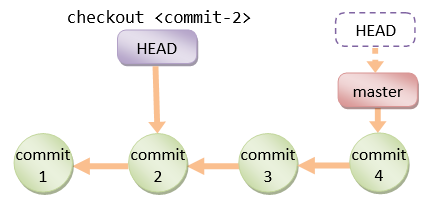
\includegraphics[width=.4\textwidth]{img/detached}
		\begin{itemize}
			\item I commit effettuati in questa modalità verranno scartati
			\item Per tornare alla modalità ``attached'', è necessario effettuare un checkout con il nome del branch
			\begin{itemize}
				\item Il nome del branch punta sempre all'ultimo commit su quella linea di sviluppo
				\item Ad esempio: \texttt{git checkout master}
			\end{itemize}
		\end{itemize}
	\end{block}
	\begin{block}{Esercizio}	
		Premessa: si osservi lo stato del repository con \texttt{git status} \textbf{prima e dopo ogni operazione}, assicurandosi di capire appieno l'output fornito da Git
		\begin{itemize}
			\item Si recuperi il file \texttt{junk.txt} da tre commit fa (\texttt{HEAD\textasciitilde{}2})
			\item Si vada al primo commit, usando il suo hash
			\begin{itemize}
				\item Potete ottenerlo usando \texttt{git log}
			\end{itemize}
			\item Si torni alla cima della linea di sviluppo (\texttt{master})
			\item Si rimuova il file \texttt{junk.txt} dall'area di staging (con \texttt{reset})
			\item Si elimini il file \texttt{junk.txt}
		\end{itemize}
	\end{block}
	\begin{block}{Output atteso}
		\begin{Verbatim}[fontsize=\scriptsize]
On branch master
nothing to commit, working tree clean
		\end{Verbatim}
	\end{block}
	\begin{block}{Output atteso}
		\begin{Verbatim}[fontsize=\scriptsize]
On branch master
Changes to be committed:
  (use "git reset HEAD <file>..." to unstage)

        new file:   junk.txt


		\end{Verbatim}
	\end{block}
	\begin{block}{Output atteso}
		\begin{Verbatim}[fontsize=\scriptsize]
A       junk.txt
Note: checking out '19aa252373d1e44897233bf5b733cf82019cd5bf'.

You are in 'detached HEAD' state. You can look around, make experimental
changes and commit them, and you can discard any commits you make in this
state without impacting any branches by performing another checkout.

If you want to create a new branch to retain commits you create, you may
do so (now or later) by using -b with the checkout command again. Example:

  git checkout -b <new-branch-name>

HEAD is now at 19aa252... Create HelloWorld
		\end{Verbatim}
	\end{block}
	\begin{block}{Output atteso}
		\begin{Verbatim}[fontsize=\scriptsize]
HEAD detached at 19aa252
Changes to be committed:
  (use "git reset HEAD <file>..." to unstage)

        new file:   junk.txt

Untracked files:
  (use "git add <file>..." to include in what will be committed)

        bin/

		\end{Verbatim}
	\end{block}
	\begin{block}{Output atteso}
		\begin{Verbatim}[fontsize=\scriptsize]
A       junk.txt
Previous HEAD position was 19aa252... Create HelloWorld
Switched to branch 'master
		\end{Verbatim}
	\end{block}
	\begin{block}{Output atteso}
		\begin{Verbatim}[fontsize=\scriptsize]
On branch master
Changes to be committed:
  (use "git reset HEAD <file>..." to unstage)

        new file:   junk.txt

		\end{Verbatim}
	\end{block}
	\begin{block}{Output atteso}
		\begin{Verbatim}[fontsize=\scriptsize]
On branch master
Untracked files:
  (use "git add <file>..." to include in what will be committed)

        junk.txt

nothing added to commit but untracked files present (use "git add" to track)
		\end{Verbatim}
	\end{block}
	\begin{block}{Output atteso}
		\begin{Verbatim}[fontsize=\scriptsize]
On branch master
nothing to commit, working tree clean
		\end{Verbatim}
	\end{block}
	\begin{block}{Spiegazione dell'output}
		\begin{itemize}
			\item Si noti che Git cerca di non cancellare le modifiche non salvate in un commit quando si naviga la storia (il file \texttt{junk.txt} non viene cancellato)
			\item In caso di conflitti, si rifiuterebbe di cambiare commit
			\item Si risolve cancellando le modifiche fatte o creando un nuovo commit, in modo da tornare allo stato di ``\texttt{working tree clean}''
		\end{itemize}
	\end{block}
\end{frame}

\subsection{Gestione di più linee di sviluppo}

\begin{frame}[allowframebreaks,fragile]{Creazione di nuove linee di sviluppo (branching)}
	\begin{block}{In generale}
		Vogliamo poter sviluppare su più linee
		\begin{itemize}
			\item Ad esempio perché stiamo per sviluppare una funzionalità che non sapremo se e quando completeremo, ma nel frattempo il nostro software va comunque manutenuto
			\item Ad esempio perché vogliamo sviluppare qualcosa a partire da una versione più vecchia (ossia, salvare i commit effettuati in modalità ``detached \texttt{HEAD}''
		\end{itemize}
	\end{block}
	\begin{block}{In Git}
		Il sottocomando \texttt{checkout} consente di creare passare di branch in branch, e di crearne di nuovi tramite l'opzione \texttt{-b}
		\begin{itemize}
			\item \texttt{git checkout -b branchname}
			\begin{itemize}
				\item Crea un nuovo branch di nome \texttt{branchname}
				\item I nuovi commit apparterranno a quel branch
			\end{itemize}
			\item \texttt{git checkout branchname}
			\begin{itemize}
				\item Passa dal branch corrente al branch \texttt{branchname}
				\item Questo in realtà è un ripasso di quanto detto un attimo fa...
			\end{itemize}
		\end{itemize}
		Il sottocomando \texttt{branch} consente di visualizzare i branch
		\begin{itemize}
			\item \texttt{git branch}
			\begin{itemize}
				\item Stampa i branch, mostrando con \texttt{*} quello corrente.
			\end{itemize}
		\end{itemize}
		L'opzione \texttt{--all} di \texttt{git log} visualizza la storia per tutti i branch
		\begin{itemize}
			\item \texttt{git log --all --graph}
		\end{itemize}
	\end{block}
	\begin{block}{Esercizio}	
		\textbf{Premessa}: si osservi e comprenda lo stato del repository con \texttt{git status} \textbf{prima e dopo ogni operazione} di modifica di file o \texttt{commit}
		\begin{itemize}
			\footnotesize
			\item Si visualizzino i branch disponibili
			\item Si crei un nuovo branch di nome \texttt{feature-readme}
			\item Si visualizzino i branch disponibili
			\item Si crei un nuovo file \texttt{README.md}, con del testo semplice
			\item Si aggiunga \texttt{README.md} alla staging area
			\item Si effettui il commit
			\item Si passi al branch \texttt{master}
			\item Si modifichi la stampa di \texttt{HelloWorld.java}
			\item Si aggiunga \texttt{HelloWorld.java} alla staging area
			\item Si effettui il commit
			\item Si visualizzi la storia dei commit su tutti i branch
		\end{itemize}
	\end{block}
	\begin{block}{Output atteso}
		\begin{Verbatim}[fontsize=\scriptsize]
* master
		\end{Verbatim}
	\end{block}
	\begin{block}{Output atteso}
		\begin{Verbatim}[fontsize=\scriptsize]
Switched to a new branch 'feature-readme'
		\end{Verbatim}
	\end{block}
	\begin{block}{Output atteso}
		\begin{Verbatim}[fontsize=\scriptsize]
* feature-readme
  master
		\end{Verbatim}
	\end{block}
	\begin{block}{Output atteso}
		\begin{Verbatim}[fontsize=\scriptsize]
On branch feature-readme
nothing to commit, working tree clean
		\end{Verbatim}
	\end{block}
	\begin{block}{Output atteso}
		\begin{Verbatim}[fontsize=\scriptsize]
On branch feature-readme
Untracked files:
  (use "git add <file>..." to include in what will be committed)

        README.md

nothing added to commit but untracked files present (use "git add" to track)
		\end{Verbatim}
	\end{block}
	\begin{block}{Output atteso}
		\begin{Verbatim}[fontsize=\scriptsize]
On branch feature-readme
Changes to be committed:
  (use "git reset HEAD <file>..." to unstage)

        new file:   README.md

		\end{Verbatim}
	\end{block}
	\begin{block}{Output atteso}
		\begin{Verbatim}[fontsize=\scriptsize]
[feature-readme 9261ec2] Add README.md file
 1 file changed, 1 insertion(+)
 create mode 100644 README.md
		\end{Verbatim}
	\end{block}
	\begin{block}{Output atteso}
		\begin{Verbatim}[fontsize=\scriptsize]
On branch feature-readme
nothing to commit, working tree clean
		\end{Verbatim}
	\end{block}
	\begin{block}{Output atteso}
		\begin{Verbatim}[fontsize=\scriptsize]
Switched to branch 'master'
		\end{Verbatim}
	\end{block}
	\begin{block}{Output atteso}
		\begin{Verbatim}[fontsize=\scriptsize]
On branch master
nothing to commit, working tree clean
		\end{Verbatim}
	\end{block}
	\begin{block}{Output atteso}
		\begin{Verbatim}[fontsize=\scriptsize]
On branch master
Changes not staged for commit:
  (use "git add <file>..." to update what will be committed)
  (use "git checkout -- <file>..." to discard changes in working directory)

        modified:   src/HelloWorld.java

no changes added to commit (use "git add" and/or "git commit -a")
		\end{Verbatim}
	\end{block}
	\begin{block}{Output atteso}
		\begin{Verbatim}[fontsize=\scriptsize]
On branch master
Changes to be committed:
  (use "git reset HEAD <file>..." to unstage)

        modified:   src/HelloWorld.java

		\end{Verbatim}
	\end{block}
	\begin{block}{Output atteso}
		\begin{Verbatim}[fontsize=\scriptsize]
[master 56aa7aa] Modify HelloWorld
 1 file changed, 1 insertion(+), 1 deletion(-)
		\end{Verbatim}
	\end{block}
	\begin{block}{Output atteso}
		\begin{Verbatim}[fontsize=\scriptsize]
On branch master
nothing to commit, working tree clean
		\end{Verbatim}
	\end{block}
	\begin{block}{Output atteso}
		\begin{Verbatim}[fontsize=\tiny]
* commit 56aa7aaad47026911c2aa2b026f33293c3b4fe31
| Author: Danilo Pianini <danilo.pianini@unibo.it>
| Date:   Thu Oct 20 15:47:57 2016 +0200
| 
|     Modify HelloWorld
|    
| * commit 9261ec24cfb56d7cd7ecc67d4eaa8add9c44b3ff
|/  Author: Danilo Pianini <danilo.pianini@unibo.it>
|   Date:   Thu Oct 20 15:43:50 2016 +0200
|   
|       Add README.md file
|  
* commit 47b5f2fb9f5300dc8bc530ce45d37a86a0436755
| Author: Danilo Pianini <danilo.pianini@unibo.it>
| Date:   Wed Oct 19 16:46:21 2016 +0200
| 
|     Remove the trash
|  
* commit 4d086a9b0d2139f0cd300d329f532a2c464304c7
| Author: Danilo Pianini <danilo.pianini@unibo.it>
| Date:   Wed Oct 19 16:45:28 2016 +0200
| 
|     move junk to trash

... CONTINUA!
		\end{Verbatim}
	\end{block}
\end{frame}

\begin{frame}[allowframebreaks,fragile]{Unione di più linee di sviluppo (merge)}
	\begin{block}{In generale}
		Vogliamo poter unire due linee di sviluppo in una sola
		\begin{itemize}
			\item Abbiamo sviluppato in un branch separato una nuova funzionalità, ora è pronta e vogliamo unirla al resto
		\end{itemize}
	\end{block}
	\begin{block}{In Git}
		Il sottocomando \texttt{merge} consente di unire due branch
		\begin{itemize}
			\item \texttt{git merge branchname}
			\begin{itemize}
				\item Tenta di unire le modifiche di \texttt{branchname} al branch corrente
				\item Prima di effettuare il merge, è necessario spostarsi sul branch destinazione (con \texttt{checkout})
				\item Se non ci sono conflitti, tutti i commit di \texttt{branchname} vengono aggiunti al branch corrente
				\item Viene creato un nuovo commit (merge commit)
				\item È buona norma non cambiare il messaggio di commit predefinito
				\item La risoluzione dei conflitti sarà uno dei temi del prossimo laboratorio
			\end{itemize}
			\item \texttt{git branch -d branchname}
			\begin{itemize}
				\item Elimina il branch \texttt{branchname}
				\item Se un branch non dovesse più servire, ad esempio perché tutte le sue modifiche sono state merse in un altro branch, è possibile rimuoverlo.
			\end{itemize}
		\end{itemize}
	\end{block}
	\begin{block}{Esercizio}	
		\textbf{Premessa}: si osservi e comprenda lo stato del repository con \texttt{git status} \textbf{prima e dopo ogni operazione} di modifica di file o \texttt{merge}
		\begin{itemize}
			\footnotesize
			\item Si visualizzino i branch disponibili, ci si assicuri di essere su \texttt{master}
			\item Si faccia il merge di \texttt{feature-readme}
			\item Si visualizzino i file del repository con \texttt{ls -ahl} (Unix) o \texttt{dir} (Windows)
			\item Si visualizzi la storia dei commit su tutti i branch
			\item Si elimini il branch \texttt{feature-readme}
			\item Si visualizzino i branch disponibili
			\item Si visualizzi la storia dei commit su tutti i branch
		\end{itemize}
	\end{block}
	\begin{block}{Output atteso}
		\begin{Verbatim}[fontsize=\scriptsize]
  feature-readme
* master
		\end{Verbatim}
	\end{block}
	\begin{block}{Output atteso}
		\begin{Verbatim}[fontsize=\scriptsize]
On branch master
nothing to commit, working tree clean
		\end{Verbatim}
	\end{block}
	\begin{block}{Output atteso}
		\begin{Verbatim}[fontsize=\scriptsize]
Merge made by the 'recursive' strategy.
 README.md | 1 +
 1 file changed, 1 insertion(+)
 create mode 100644 README.md
		\end{Verbatim}
	\end{block}
	\begin{block}{Output atteso}
		\begin{Verbatim}[fontsize=\scriptsize]
On branch master
nothing to commit, working tree clean
		\end{Verbatim}
	\end{block}
	\begin{block}{Output atteso}
		\begin{Verbatim}[fontsize=\scriptsize]
total 2.0M
drwxr-xr-x 5 danysk users 4.0K Oct 20 16:15 .
drwxr-xr-x 6 danysk users 2.0M Oct 20 15:56 ..
drwxr-xr-x 2 danysk users 4.0K Oct 19 16:22 bin
drwxr-xr-x 8 danysk users 4.0K Oct 20 16:15 .git
-rw-r--r-- 1 danysk users    5 Oct 19 18:55 .gitignore
-rw-r--r-- 1 danysk users   25 Oct 20 16:15 README.md
drwxr-xr-x 2 danysk users 4.0K Oct 19 16:00 src
		\end{Verbatim}
	\end{block}
	\begin{block}{Output atteso}
		\begin{Verbatim}[fontsize=\tiny]
*   commit b68c8a48dc24bd1d948c2ac4409d8d91a000b8b6
|\  Merge: 56aa7aa 9261ec2
| | Author: Danilo Pianini <danilo.pianini@unibo.it>
| | Date:   Thu Oct 20 16:15:47 2016 +0200
| | 
| |     Merge branch 'feature-readme'
| |   
| * commit 9261ec24cfb56d7cd7ecc67d4eaa8add9c44b3ff
| | Author: Danilo Pianini <danilo.pianini@unibo.it>
| | Date:   Thu Oct 20 15:43:50 2016 +0200
| | 
| |     Add README.md file
| |   
* | commit 56aa7aaad47026911c2aa2b026f33293c3b4fe31
|/  Author: Danilo Pianini <danilo.pianini@unibo.it>
|   Date:   Thu Oct 20 15:47:57 2016 +0200
|   
|       Modify HelloWorld
|  
* commit 47b5f2fb9f5300dc8bc530ce45d37a86a0436755
| Author: Danilo Pianini <danilo.pianini@unibo.it>
| Date:   Wed Oct 19 16:46:21 2016 +0200
| 
|     Remove the trash
|  

...CONTINUA!
		\end{Verbatim}
	\end{block}
	\begin{block}{Output atteso}
		\begin{Verbatim}[fontsize=\scriptsize]
Deleted branch feature-readme (was 9261ec2).
		\end{Verbatim}
	\end{block}
	\begin{block}{Output atteso}
		\begin{Verbatim}[fontsize=\scriptsize]
* master
		\end{Verbatim}
	\end{block}
	\begin{block}{Output atteso}
		\begin{Verbatim}[fontsize=\tiny]
*   commit b68c8a48dc24bd1d948c2ac4409d8d91a000b8b6
|\  Merge: 56aa7aa 9261ec2
| | Author: Danilo Pianini <danilo.pianini@unibo.it>
| | Date:   Thu Oct 20 16:15:47 2016 +0200
| | 
| |     Merge branch 'feature-readme'
| |   
| * commit 9261ec24cfb56d7cd7ecc67d4eaa8add9c44b3ff
| | Author: Danilo Pianini <danilo.pianini@unibo.it>
| | Date:   Thu Oct 20 15:43:50 2016 +0200
| | 
| |     Add README.md file
| |   
* | commit 56aa7aaad47026911c2aa2b026f33293c3b4fe31
|/  Author: Danilo Pianini <danilo.pianini@unibo.it>
|   Date:   Thu Oct 20 15:47:57 2016 +0200
|   
|       Modify HelloWorld
|  
* commit 47b5f2fb9f5300dc8bc530ce45d37a86a0436755
| Author: Danilo Pianini <danilo.pianini@unibo.it>
| Date:   Wed Oct 19 16:46:21 2016 +0200
| 
|     Remove the trash
|  

...CONTINUA!
		\end{Verbatim}
	\end{block}
\end{frame}

\begin{frame}{Conclusioni}
	\begin{itemize}
		\item Avete in mano uno strumento molto potente
		\item Usatelo sempre d'ora in poi
		\item A partire da questo laboratorio!
		\begin{itemize}
			\item Effettuate almeno un commit alla fine di ogni esercizio prima di chiamarci per correggere
			\item Se ve ne servono di più, fatene di più!
		\end{itemize}
	\end{itemize}
	\begin{block}{Nei prossimi laboratori}
		\begin{itemize}
			\item Impareremo ad usare git per lavorare in modo efficace con un team di persone
			\item Impareremo a scambiarci commit via Internet
			\item Lo useremo per ottenere le esercitazioni (bye bye zip files)
		\end{itemize}
	\end{block}
	\begin{block}{Nel progetto d'esame}
		\begin{itemize}
			\item Andrà consegnato sotto forma di repository Git o Mercurial
			\item L'abilità nell'uso del DVCS sarà parte della valutazione
		\end{itemize}
	\end{block}
\end{frame}


\end{document}

\begin{frame}{Branching}
	\begin{block}{Il concetto di branching}
		Dal momento in cui possiamo andare indietro nella storia ed effettuare nuovi commit, abbiamo la possibilità di fare \textit{branching}: abbiamo più di una linea di sviluppo che viene portata avanti!
		\begin{center}
			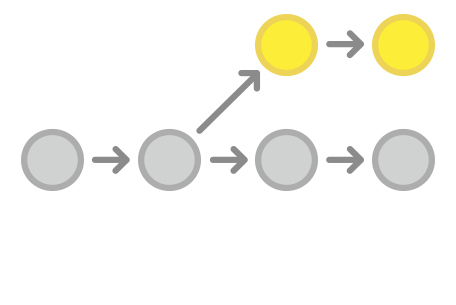
\includegraphics[width=0.6\textwidth]{img/branch}
		\end{center}
	\end{block}
\end{frame}

\begin{frame}{Branching esplicito vs. implicito}
	In Mercurial, a seconda che si dia o meno un nuovo nome al branch, è possibile che:
	\begin{enumerate}
		\item Si avvii una nuova linea di sviluppo senza dichiararla. In questo caso, Mercurial tratta la situazione come \textbf{un singolo branch con più teste di sviluppo}. È una situazione che si vuole evitare, nel caso in cui accada si vuole sempre riunire le teste in una unica (merge). \\ \alert{Nota}: git proibisce espressamente questo genere di branching
		\item Si dichiara che si sta avviando una nuova linea di sviluppo e le si dà un nome. Viene creato un cosiddetto ``named branch'', il DVCS offre comandi che supportano la creazione di più linee ed il passaggio da una all'altra.
	\end{enumerate}
\end{frame}

\begin{frame}{Branching implicito: visualizzazione delle teste}
	Dal momento in cui possiamo andare indietro nella storia ed effettuare nuovi commit, abbiamo la possibilità di fare \textit{branching implicito}: potremmo trovarci nella situazione di avere più teste! C'è la necessità di vedere quante sono e a che punto sono.
	\begin{center}
		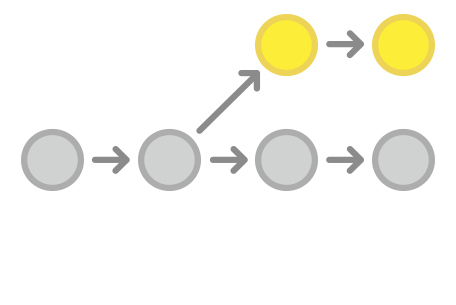
\includegraphics[width=0.6\textwidth]{img/branch}
	\end{center}
	\bl{In Mercurial}{
		\iz{
			\item \texttt{hg heads}
		}
		Mostra tutte le linee di sviluppo attualmente attive (l'output è simile a quello di \texttt{hg log}).
	}
\end{frame}

\begin{frame}{Branching esplicito}
	Per la gestione dei named branches occorrono una serie di strumenti:
	\begin{itemize}
		\item Visualizzazione del branch corrente
		\item Creazione di un nuovo branch
% 		\item Chiusira di un branch non più usato, ad esempio perché è stato usato per sviluppare una nuova feature, ed ora la feature è pronta per essere inserita nella linea di sviluppo principale.
		\item Passaggio ad un altro branch
		\item Merge di due branch
	\end{itemize}
\end{frame}

\begin{frame}{Branching: operazioni di base}
	\begin{block}{Visualizzare il branch corrente}
		\begin{center}
			\texttt{hg branch}
		\end{center}
		Visualizza il nome del branch corrente. Se non si è creato alcun branch manualmente, esiste un solo branch chiamato \texttt{default}
	\end{block}
	\begin{block}{Creazione di un nuovo branch}
		\begin{center}
			\texttt{hg branch nome\_del\_nuovo\_branch}
		\end{center}
		Assegna il nome \texttt{nome\_del\_nuovo\_branch} al branch corrente: a partire dal commit successivo, si lavorerà su \texttt{nome\_del\_nuovo\_branch}
	\end{block}
	\begin{block}{Passaggio ad un altro branch}
		\begin{center}
			\texttt{hg update nome\_del\_branch --clean}
		\end{center}
		Passa al branch \texttt{nome\_del\_branch}. Se si attiva l'opzione texttt{--clean}, verranno aggiornati anche i file nella working directory
	\end{block}
\end{frame}


\fr{Merge}{
	\bl{In generale}{
		Dal momento in cui possiamo avere più branch, oppure un branch con più teste, abbiamo necessità di uno strumento che ci consenta di riunirle. Ad esempio:
		\begin{itemize}
			\item Abbiamo creato un nuovo branch per testare una nuova feature senza danneggiare il nostro software funzionante. Ora tutto è a posto, e vogliamo integrare le modifiche nella ``mainline''
			\item Siamo andati indietro nella storia, abbiamo visto un errore e l'abbiamo corretto senza fare un nuovo branch. Dopo il commit, ci troviamo un branch con due teste, e vogliamo riunirle.
		\end{itemize}
		\begin{center}
			\centering{}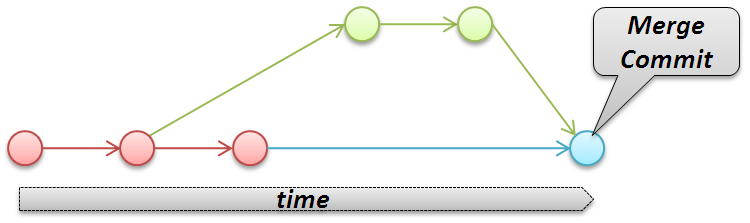
\includegraphics[width=0.6\textwidth]{img/merge}
		\end{center}
	}
}

\begin{frame}{Merge di più teste in Mercurial}
	Nel caso in cui vi siano più teste nel branch corrente, il comando
	\begin{center}
		\texttt{hg merge}
	\end{center}
	Tenta di unirle.
	Una volta che il merge è completo, per registrare le modifiche è necessario eseguire un \texttt{commit}.

	Grazie al tracciamento differenziale, esistono algoritmi molto potenti che consentono di risolvere automaticamente la maggior parte dei conflitti. È comunque possibile che, in caso di modifiche sullo stesso file, si generi un \emph{conflitto di merge}. Quando capita, il conflitto andrà risolto manualmente.
\end{frame}

\begin{frame}{Merge di più branch in Mercurial}
	Nel caso di più branch, si fa un'operazione analoga. Supponiamo di avere due branch: uno chiamato \texttt{mainline}, dove teniamo lo sviluppo principale, ed uno chiamato \texttt{feature}, dove abbiamo sviluppato una nuova funzionalità che adesso vogliamo portare sul nostro branch principale.
	\begin{enumerate}
	 \item Si passa al branch ``destinazione'', ossia quello che consideriamo essere il principale. Se si è già nel branch corretto, e se non ci sono modifiche pendenti, non è necessario.
		\begin{itemize}
			\item \texttt{hg update mainline --clean}
		\end{itemize}
	 \item Si fa il merge del branch che contiene le nuove feature in modo analogo a quello che abbiamo fatto nel caso di più teste:
		\begin{itemize}
			\item \texttt{hg merge feature}
			\item \texttt{hg commit -m "Merge feature into mainline"}
		\end{itemize}
	 \item Si segnala che il branch precedente non sarà più usato ``chiudendolo'' con uno speciale commit:
		\begin{itemize}
			\item \texttt{hg update feature}
			\item \texttt{hg commit --close-branch -m "Close branch feature"}
			\item \texttt{hg update mainline}
		\end{itemize}
	\end{enumerate}
\end{frame}

\begin{frame}{Esercizio}
	Provate a svolgere l'esercizio 0 dell'esercitazione. Troverete un file di istruzioni che vi spiegherà dettagliatamente il da farsi.
\end{frame}


\fr{Nella prossima puntata}{
	\iz {
		\item Merge conflicts e loro risoluzione
		\item Servizi di hosting per repository Mercurial e Git
		\item Lavoro parallelo in gruppo con DVCS
		\item Aspetti avanzati: rebasing, bisection, cherry picking (cenni)
		\item Workflow suggeriti per sfruttare al massimo i DVCS
		\item Il menù ``Team'' di Eclipse e il plug-in HGE
	}
}

\section{Lab Startup}

\fr{Preparazione Ambiente di Lavoro 1/2}{
	\iz{
		\item Accendere il PC
		\item Loggarsi sul sito del corso
		\iz{
			\item \textcolor{blue}{\url{https://elearning-cds.unibo.it/course/view.php?id=3042}}
		}
		\item Scaricare dalla sezione \texttt{lab} del sito il file \texttt{oop1415-lab07.zip} contenente il materiale dell'esercitazione odierna
		\item Spostare il file scaricato sul Desktop
		\item Decomprimere il file usando 7zip (o un programma analogo) sul Desktop
	}
}

\fr{Preparazione Ambiente di Lavoro 2/2}{
	\iz{
		\item Copiare la cartella scompattata nel vostro workspace di Eclipse
		\iz{
			\item p.e. \texttt{C:$\backslash$Users$\backslash$<username>$\backslash$workspace}
		}
		\item Importare il progetto \texttt{OOP1415\_Lab07\_Code} con la procedura standard di importazione dei progetti
	}
}


\fr{Modalità di Lavoro}{
  \bl{}{
    \en{
      \item Gli esercizi sono divisi in package con nomi progressivi
      \item Troverete un commento con le istruzioni per ciascun esercizio
      \item Risolvere l'esercizio in autonomia
      \item Cercare di risolvere autonomamente eventuali piccoli problemi che possono verificarsi durante lo svolgimento degli esercizi
      \item \textcolor{red}{Utilizzare i test JUnit presenti nei sorgenti per il testing dell'esercizio}
      \item Contattare i docenti nel caso vi troviate a lungo bloccati nella risoluzione di uno specifico esercizio
      \item \textbf{A esercizio ultimato contattare i docenti per un rapido controllo della soluzione realizzata}
      \item Proseguire con l'esercizio seguente
    }
  }
}

%%%%%%%%%%%%%%%%%%%%%%%%%%%%%%%%%%%%%%
%%%% TO BE REUSED ON NEXT LAB %%%%%%%%
%%%%%%%%%%%%%%%%%%%%%%%%%%%%%%%%%%%%%%

\subsection{Lavorare con più repository}

\fr{Clone}{
  Esiste ovviamente la possibilità di clonare un repository già esistente, sul quale volete lavorare.\\
  \bl{il comando \texttt{clone}}{
    \texttt{clone} deve essere seguito dall'URI a cui si trova il repository che volete clonare. Può essere un repository sul vostro disco, può essere un repository che si trova online (vedremo dopo alcuni servizi di hosting), può essere un repository che si trova nella vostra rete locale.
  }
  \bl{Esempi}{
    \iz{
      \item \texttt{clone /home/user/repo1 /home/user/repo2} --- Clona un repository sul disco locale nel path specificato.
      \item \texttt{clone https://user@service.org/repo /home/user/repo2} --- Clona un repository remoto sul disco, nel path specificato, con protocollo HTTPS.
    }
    Si noti che gli URI da inserire in clone possono essere DVCS-specifici.
  }
}

\fr{Pull}{
  L'operazione di \texttt{pull} consente di prendere dati da un altro repository per inserirli nel proprio.\\
  \bl{il comando \texttt{pull}}{
    \texttt{clone} deve essere seguito dall'URI a cui si trova il repository di cui volete copiare le differenze. Ovviamente, i due repository devono avere la stessa radice, ossia avere una parte in comune.
  }
}

\fr{Push}{
  \bl{In teoria, l'operazione di \texttt{pull} è sufficiente. In pratica, no.}{
    \iz {
      \item Se il repository locale è su una macchina NATtata?
      \item Se il repository remoto è un server cui non potete accedere per fare \texttt{pull}?
    }
    Serve un meccanismo per ``spingere'' le modifiche verso un altro repository, ossia il complementare di \texttt{pull}. Tale meccanismo è \texttt{push}.
  }
}

\fr{Lavorare in parallelo}{
  \bl{Fin qui tutto molto carino...} {
   ...ma abbiamo lavorato sequenzialmente, e mai in parallelo.
  }
  Il vero vantaggio nell'uso di DVCS si ha quando si comincia a lavorare parallelamente sulla stessa cosa. 
}

\fr{Lavorare in parallelo: esempio}{
  Situazione iniziale:
  \begin{center}
    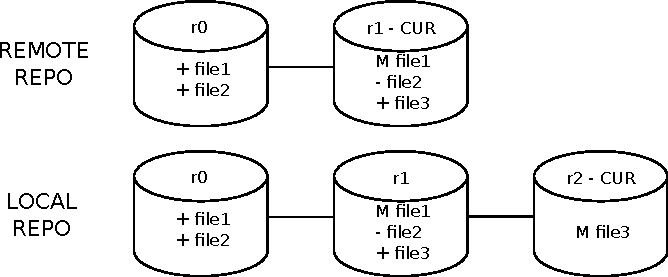
\includegraphics[width=0.99\textwidth]{img/draw5}
  \end{center}
}

\fr{Lavorare in parallelo: esempio}{
  Remote esegue:\\
  Modifica di \texttt{file2} \\
  \texttt{commit} \\
  \begin{center}
    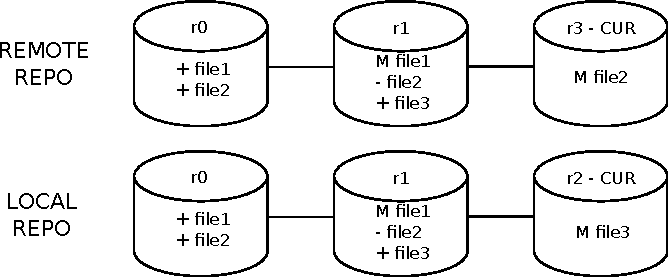
\includegraphics[width=0.99\textwidth]{img/draw7}
  \end{center}
}

\fr{Lavorare in parallelo: esempio}{
  Local esegue:\\
  \texttt{push indirizzo\_di\_remote\_repo} \\
  \texttt{commit} \\
  \begin{center}
    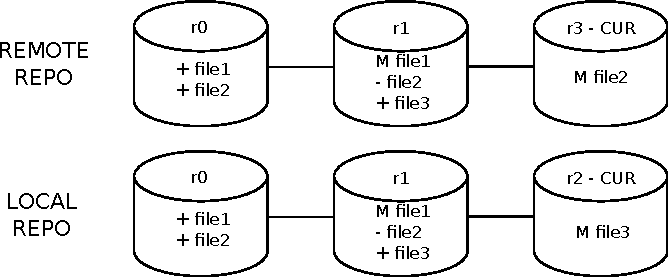
\includegraphics[width=0.99\textwidth]{img/draw7}
  \end{center}
  La push viene rifiutata: la radice dei due repository è diversa!
}

\fr{Lavorare in parallelo: esempio}{
  Local esegue:\\
  \texttt{push indirizzo\_di\_remote\_repo} \\
  \texttt{commit} \\
  \begin{center}
    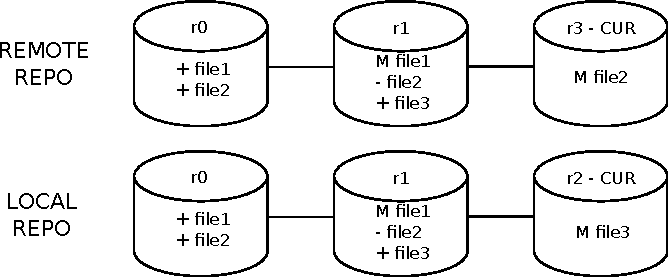
\includegraphics[width=0.99\textwidth]{img/draw7}
  \end{center}
  La push viene rifiutata: la radice dei due repository è diversa!
}

\fr{Lavorare in parallelo: esempio}{
  Local esegue:\\
  \texttt{pull indirizzo\_di\_remote\_repo} \\
  \begin{center}
    \includegraphics[width=0.7\textwidth]{img/draw8}
  \end{center}
  Il repository locale ora può essere portato anche alla versione \texttt{r3}. Nonostante ciò, le push vengono rifiutate, poiché il repository locale ha due teste!
}

\fr{Merge}{
  L'operazione di \texttt{merge} consente di unire due teste di un repository unendo le loro modifiche.
  \iz {
    \item Se le modifiche effettuate concorrentemente non toccano gli stessi files, tali modifiche sono semplicemente unite insieme.
    \item Se le modifiche toccano gli stessi files in parti diverse. il DVCS fa del suo meglio per cercare di risolvere i conflitti.
    \item Se ci sono conflitti a livello della singola linea di codice, è necessario un intervento manuale: l'utente deve selezionare le righe che vuole mantenere nella versione merged.
  }
}

\fr{Merge: esempio}{
  Situazione iniziale:\\
  \begin{center}
    \includegraphics[width=0.7\textwidth]{img/draw8}
  \end{center}
}

\fr{Merge: esempio}{
  Local esegue:\\
  \texttt{merge} \\
  \begin{center}
    \includegraphics[width=0.99\textwidth]{img/draw9}
  \end{center}
  Ora è possibile effettuare push: c'è una sola testa!
}

\fr{Merge: esempio}{
  Local esegue:\\
  \texttt{push indirizzo\_di\_remote\_repo} \\
  \begin{center}
    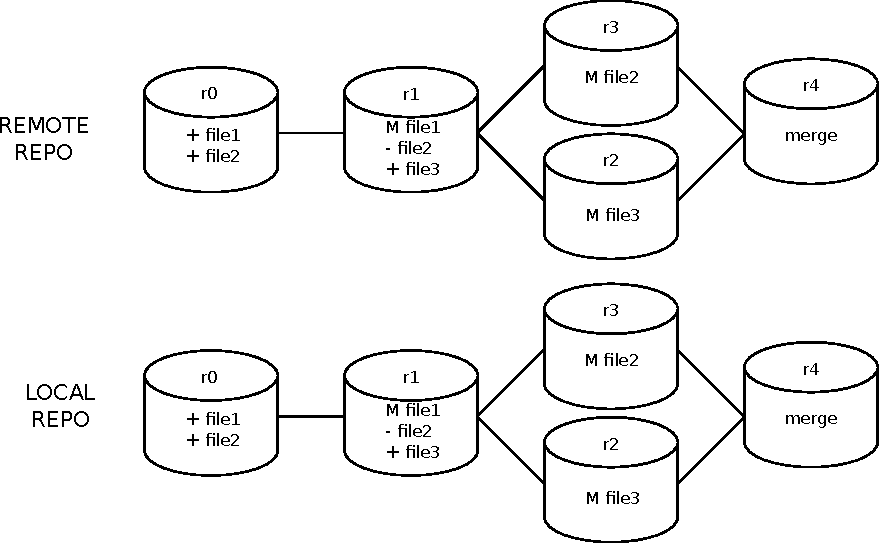
\includegraphics[width=0.8\textwidth]{img/draw10}
  \end{center}
  Ora è possibile effettuare push: c'è una sola testa!
}

\fr{Aspetti avanzati}{
  \bl{Branching}{
    Creazione volontaria di più ``teste''. Si usa, ad esempio, quando si vuole sviluppare una funzionalità sperimentale, e integrarla solo successivamente.
  }
  \bl{Rebasing}{
    Procedura alternativa al merge, in cui i due commit, invece di essere fusi, vengono messi in sequenza.
  }
  \bl{Cherry picking}{
    Pull di un singolo commit. Spesso utilizzato quando si desidera avere un bugfix che si trova in un altro branch, ma non tutto il resto.
  }
  \bl{Bisection}{
    Strategia per scoprire bug in maniera automatizzata, testando il software a varie versioni (ricerca dicotomica). Una volta trovata la prima versione dove il bug si verifica, si controllano commit message e le differenze.
  }
}

\subsection{Un DVCS: Mercurial}

\fr{Plugin Eclipse}{
  È disponibile anche un plugin per Eclipse, che semplifica molto la gestione del repository quando sviluppate con l'IDE.
  \bl{Installazione}{
    \begin{enumerate}
     \item Help $\Rightarrow$ Install new software...
     \item Inserire l'indirizzo \url{http://hge.javaforge.com/mercurialeclipse-snapshots} e premere invio
     \item Selezionare il plugin che viene caricato 
     \item Next
     \item Accettare le eventuali licenze
     \item Accettare l'eventuale richiesta di installazione di software non firmato
     \item Riavviare Eclipse
    \end{enumerate}
  }
}

\fr{Uso del plugin di eclipse}{
  \iz{
    \item   Una volta installato, sarà possibile utilizzare Mercurial dalla veste grafica interna ad Eclipse. I comandi sono accessibili nel sotto-menu ``Team''.
    \item La prima operazione da fare è attivare Mercurial nel progetto, tramite Team $\Rightarrow$ Share. Da questo momento sarà possibile utilizzare tutte le funzioni di Mercurial.
    \item Nota: ricordatevi \textbf{sempre} di mettere correttamente il nome del committer quando eseguite un commit. Il formato è\\ Nome Cognome \textless{}indirizzo@email.qui\textgreater{}
  }
}

\subsection{Servizi di hosting}

\fr{Servizi di hosting}{
  \iz{
    \item Esistono diversi servizi online che vi consentono di mantenere una copia remota del repository
    \item Perché dovreste avere una copia remota?
    \iz{
      \item Sicurezza
      \item Condivisione con altri
      \item Semplificazione dello sviluppo in gruppo
    }
    \item Questi servizi spesso vi forniscono strumenti potenti
    \iz{
      \item Possibilità di visualizzare la storia dello sviluppo
      \item Forks
      \item Pull requests
      \item Commenti per-linea di codice
    }
  }
  I due più comuni sono GitHub (\url{https://github.com/}) e Bitbucket (\url{https://bitbucket.org/}). Il primo supporta solamente git, mentre il secondo supporta sia git che Mercurial.
}

\fr{Bitbucket}{
  \iz {
    \item Vi consigliamo di usare Bitbucket, lo utilizziamo anche noi per le vostre slides e esercitazioni.
    \item Se vi iscrivete utilizzando la mail istituzionale, riceverete un account illimitato gratuitamente (il prezzo dell'account illimitato si aggira sui 120\$ al mese)
  }
}

\fr{Bitbucket: project overview, RSS}{
  \begin{center}
    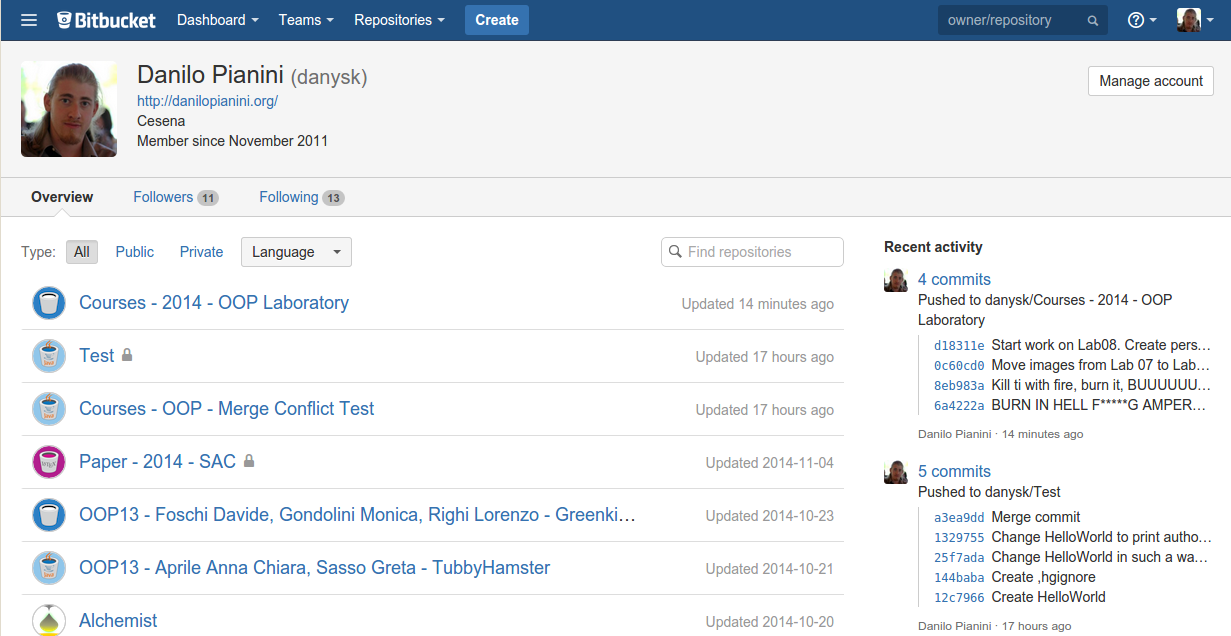
\includegraphics[width=0.99\textwidth]{img/bitbucket0}
  \end{center}
}

\fr{Bitbucket: source navigation}{
  \begin{center}
    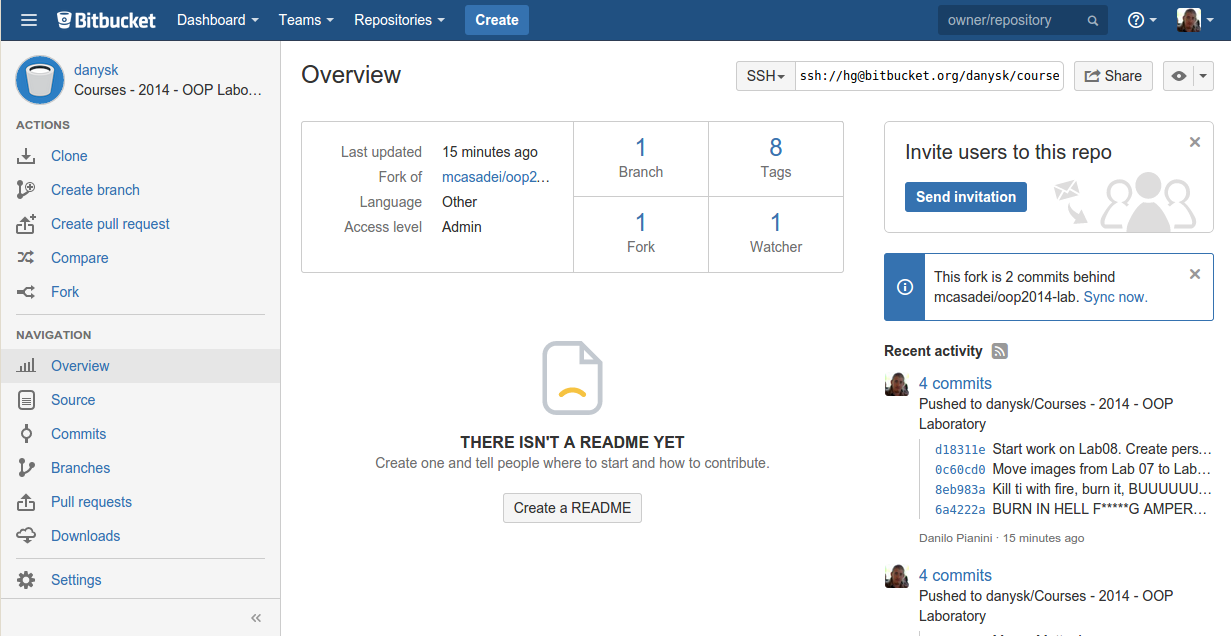
\includegraphics[width=0.99\textwidth]{img/bitbucket1}
  \end{center}
}
\fr{Bitbucket: development history}{
  \begin{center}
    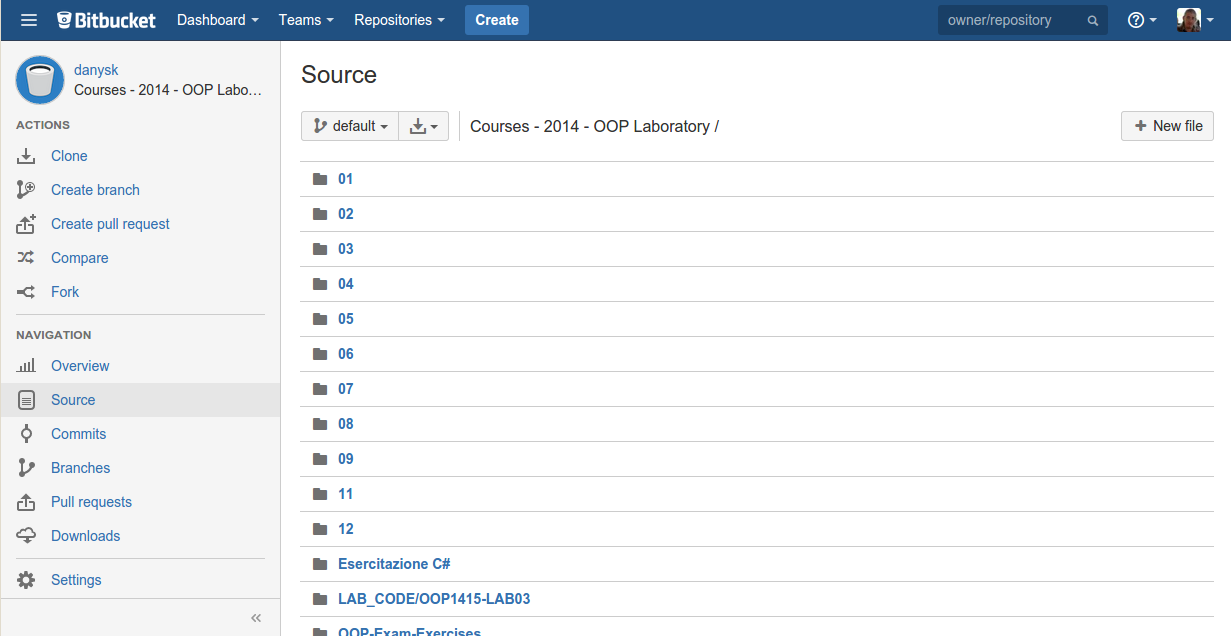
\includegraphics[width=0.99\textwidth]{img/bitbucket2}
  \end{center}
}

\fr{Bitbucket: bug tracker and wiki}{
  \begin{center}
    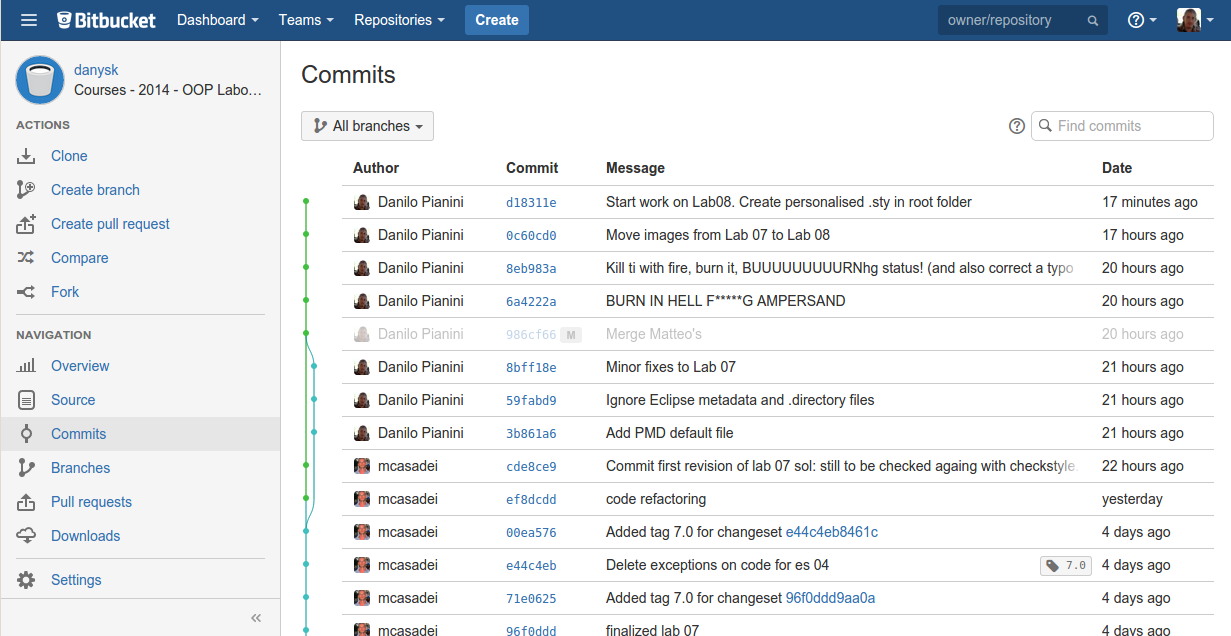
\includegraphics[width=0.99\textwidth]{img/bitbucket3}
  \end{center}
}

\fr{Bitbucket: download page}{
  \begin{center}
    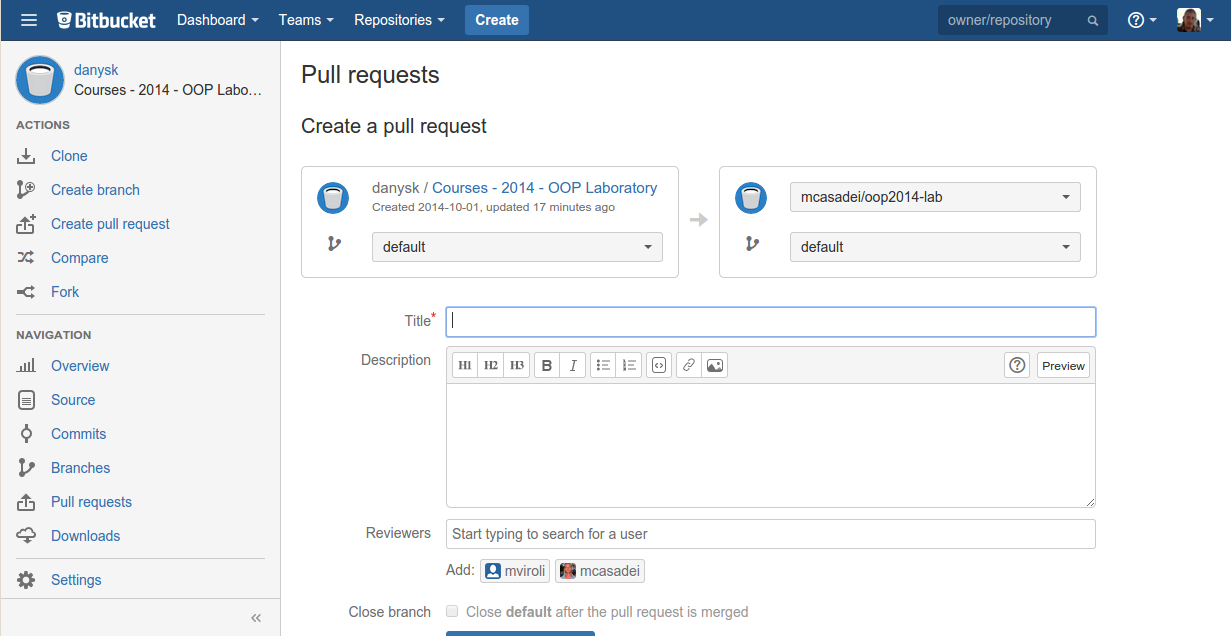
\includegraphics[width=0.99\textwidth]{img/bitbucket4}
  \end{center}
}

\fr{Bitbucket: Pull requests, Compare e Fork}{
  \begin{center}
    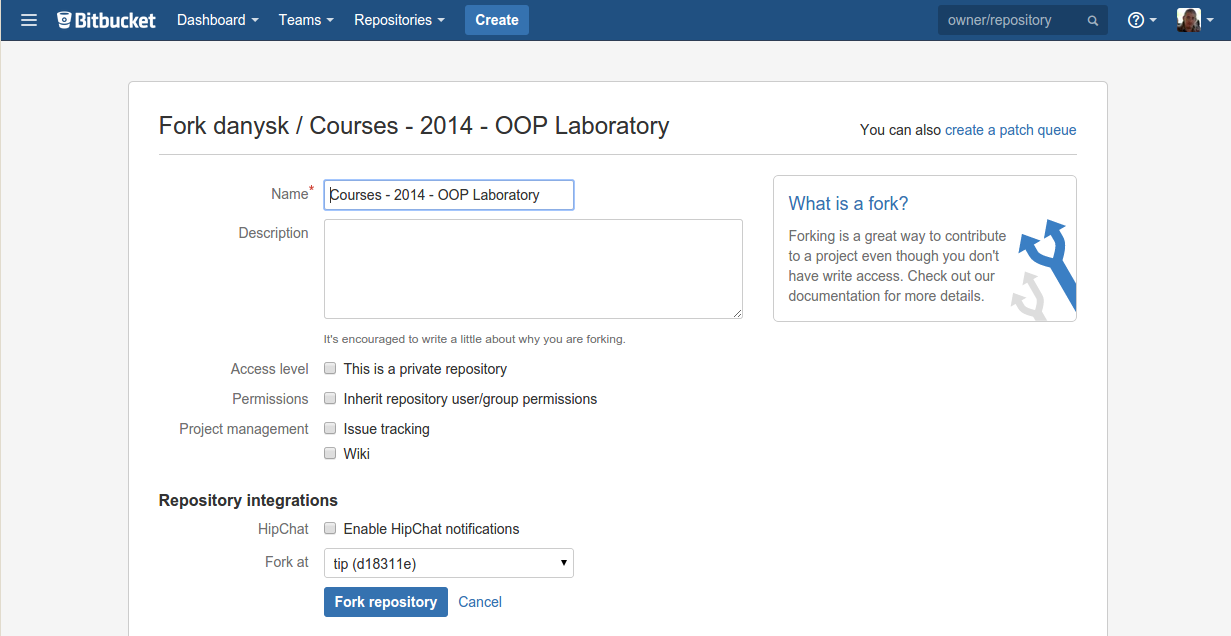
\includegraphics[width=0.99\textwidth]{img/bitbucket5}
  \end{center}
}


\subsection{Workflow suggeriti}
\fr{Esercizio con Mercurial} {
  Utilizzando i comandi visti finora, si svolgano i seguenti passi:
  \begin{enumerate}
   \item Si inizializzi un nuovo repository
   \item Si creino due file di testo e si aggiungano al repository
   \item Si usi \texttt{hg status} per vedere lo stato del repository
   \item Si faccia un commit
   \item Si usi \texttt{hg log} per vedere la storia del repository
   \item Si cancellino i due file dal file system (non dal repository!)
   \item Si ripristinino i due file cancellati sfruttando il comando \texttt{hg update}
   \item Si cloni il repository in un'altra cartella usando \texttt{hg clone}
   \item Si modifichi, nel nuovo repository, uno dei file
   \item Si faccia un commit nel nuovo repository
   \item Si usi \texttt{hg push} per spingere la modifica sul vecchio repository
  \end{enumerate}
  A casa, si facciano ulteriori prove, anche utilizzando il plug-in di Eclipse e creando un repository su Bitbucket. Si sfrutti il forum del corso nel caso si incontrino problemi.
}

